\section{Component Execution Semantics}
\label{sec:ROSMOD}

A \emph{component operation} is an abstraction for the different tasks undertaken by a component. These tasks are implemented by the component's executor code written by the developer. Application developers provide the functional, \emph{business-logic} code that implements operations on the state variables e.g. a proportional-integral-derivative controller operation could receive the current state of dynamic variables from a \emph{Sensor} Component, and using the relevant gains, calculate a new state to which an \emph{Actuator} component should progress the system. In order to service interactions with the underlying framework and with other components, every component is associated with a \emph{message queue}. This queue holds instances of operations ('messages') that are ready for execution and need to be serviced by the component. These operations service either interaction requests (seen on communication ports) or service requests (from the underlying framework). An example for the latter is the use of component timers that can periodically (or sporadically) activate an operation. 

To facilitate component behavior that is free of deadlocks and race conditions, the component's execution is handled by a single thread. Operations in the message queue are therefore scheduled one at a time under a non-preemptive policy. A component dispatcher thread dequeues the next ready operation from the component message queue. This operation is scheduled for execution on a component executor thread. The operation is run to completion before another operation from the queue is serviced. This single-threaded execution helps avoid synchronization primitives such as internal state variables that lead to strenuous code development. Though components that share a processor still run concurrently, each component operation is executed by a single component-specific executor thread.

\begin{figure}[ht]
	\centering
	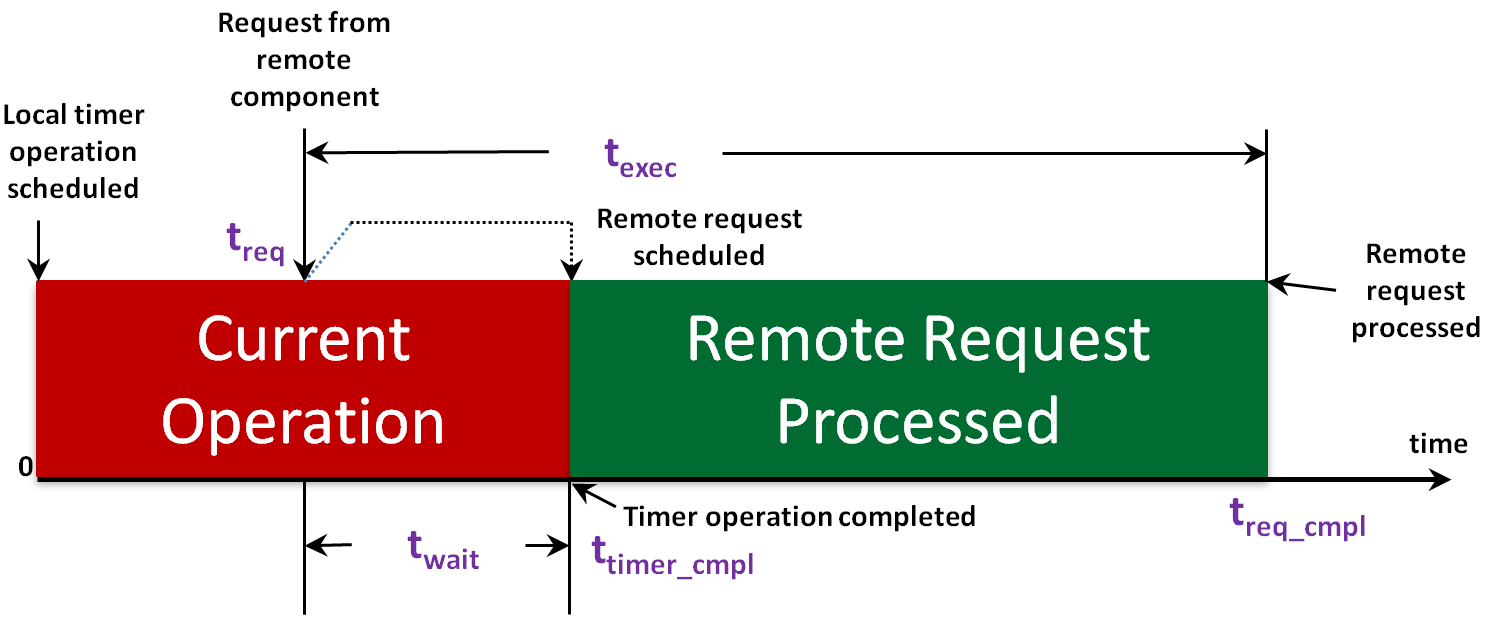
\includegraphics[width=0.5\textwidth]{cop_execution_semantics}
	\caption{Component Operation Execution Semantics: This figure shows the effects of the ROSMOD component scheduling on an incoming operation request. $t\_{req}$ represents the arrival time of a remote request. $t\_{wait}$ is the wait time of this request in the message queue while the current operation is still executing. $t\_{timer\_cmpl}$ is the time stamp at which the current operation completes executing. At this time, the remote request is finally scheduled for execution. $t\_{req\_cmpl}$ is the time stamp at which the remote request completes. The execution time, $t\_{exec}$ of this request is calculated as the difference in time stamps between $t\_{req\_cmpl}$ and $t\_{req}$.}
	\label{fig:cop_execution_semantics}
\end{figure}

Figure \ref{fig:cop_execution_semantics} shows the execution semantics of a component operation executed on a lone component executor thread. A simplifying assumption  to describe the semantics is that this component is the only component thread executing on this CPU. Assume that at $t=0$, this component is processing the expiry of a local timer. This operation is expected to complete at $t = t_{timer\_cmpl}$. However, at $t = t_{req}$, a service request is received from some remote component. Since the component operation scheduling is non-preemptive, regardless of the priority of this service, the request is not processed until $t_{timer\_cmpl}$. Therefore, the request is waiting in the message queue for $t_{wait} = t_{timer\_cmpl} - t_{req}$. At $t = t_{timer\_cmpl}$, the timer operation is marked as complete and the service request is processed. The total execution time of this service operation is calculated including the duration of the time for which this request waited in the component message queue i.e. $t_{exec} = t_{req\_cmpl} - t_{req}$. The wait times in the queue are further worsened when OS scheduling non-determinism is taken into account. There are specifically three ways in which the OS scheduling can delay operations: (1) if the application process is concurrently executing executor threads of multiple components of equal priority, then the threads are scheduled in Round-Robin fashion by the OS, (2) when mixed-criticality application processes are scheduled in tandem, the OS uses fixed-priority Round-Robin scheduling to schedule the process threads, and finally (3) temporally partitioned OS schedules further cause delays on component thread scheduling, which directly affects the scheduling and timely completion of component operations. 